% ------------------------------------------------------------------------------
% TYPO3 CMS 6.2 LTS - What's New - Chapter "Backend Changes" (English Version)
%
% @author	Michael Schams <schams.net>
% @license	Creative Commons BY-NC-SA 3.0
% @link		http://typo3.org/download/release-notes/whats-new/  
% @language	English
% ------------------------------------------------------------------------------
% Chapter: Backend Changes   
% ------------------------------------------------------------------------------
\section{Panel administracyjny}
\begin{frame}[fragile] 
	\frametitle{Panel administracyjny}

	\begin{center}\huge{Rozdział 3:}\end{center}
	\begin{center}\huge{\color{typo3darkgrey}\textbf{Zmiany w panelu administracyjnym}}\end{center}

\end{frame}

% ------------------------------------------------------------------------------
% Autofocus
% ------------------------------------------------------------------------------
% http://forge.typo3.org/issues/49228

\begin{frame}[fragile]
	\frametitle{Zmiany w panelu administracyjnym}
	\framesubtitle{Logowanie do panelu administracyjnego}

 	\begin{itemize}
		\item Autofokus w polu username w formularzu logowania do panelu administracyjnego\newline
			(HTML5 atrybut: \texttt{autofocus="autofocus"})
	\end{itemize}

	\begin{figure}
		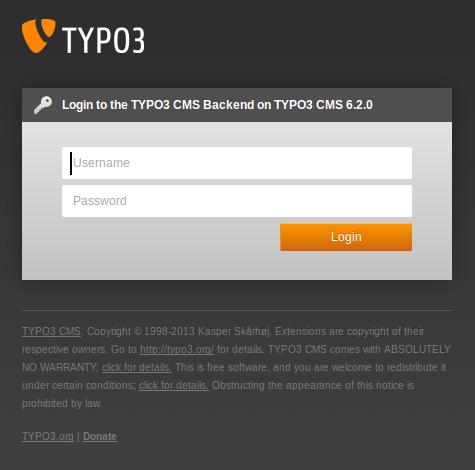
\includegraphics[width=0.4\linewidth]{Images/BackendChanges/BackendLogin.png}
	\end{figure}

\end{frame}

% ------------------------------------------------------------------------------
% Visual Appearance
% ------------------------------------------------------------------------------
% http://forge.typo3.org/issues/48376

\begin{frame}[fragile]
	\frametitle{Zmiany w panelu administracyjnym}
	\framesubtitle{Wygląd}

	\begin{columns}[T]

		\begin{column}{.5\textwidth}
			\begin{itemize}
				\item Ulepszono obsługę za pomocą techniki livening
				\item Zwiększono marginesy między modułami ("left-hand-side column")
				\item Wykorzystano 12 pikselową siatkę, którą podwojono
			\end{itemize}

			\advance\leftskip+2.5cm

			\smaller
				Po lewej: TYPO3 4.5\newline
				Po prawej: TYPO3 6.2
			\normalsize
		\end{column}

		\begin{column}{.5\textwidth}
			\begin{figure}\vspace*{-0.4cm}
				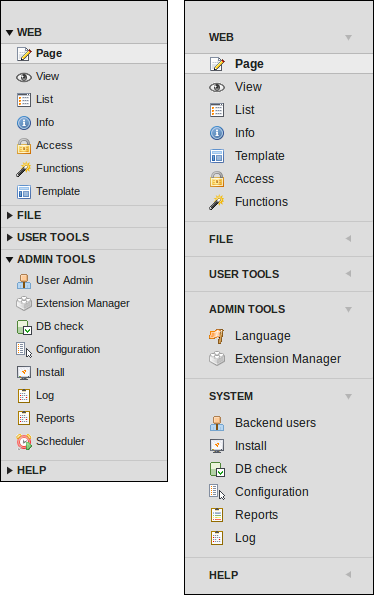
\includegraphics[width=0.6\linewidth]{Images/BackendChanges/VisualAppearance.png}
			\end{figure}
		\end{column}

	\end{columns}

\end{frame}

% ------------------------------------------------------------------------------
% Visual Appearance  
% ------------------------------------------------------------------------------

\begin{frame}[fragile]
	\frametitle{Zmiany w panelu administracyjnym}
	\framesubtitle{Wygląd}

	\begin{columns}[T]

		\begin{column}{.5\textwidth}

			\begin{itemize}
				\item Zreorganizowano moduły w lewej kolumnie.
				\item Moduł "ADMINTOOLS" podzielono na dwie części:

					\begin{itemize}
						\item \textbf{ADMINTOOLS} ("Languages" i "Extension Manager")
						\item \textbf{SYSTEM} (niskopoziomowe narzędzia, które nie pokazują 3-kolumnowej strony)
					\end{itemize}

				\item Usunięto przestarzały moduł "TypoScript Help" 

			\end{itemize}

		\end{column}

		\begin{column}{.5\textwidth}
			\begin{figure}\vspace*{-0.4cm}
				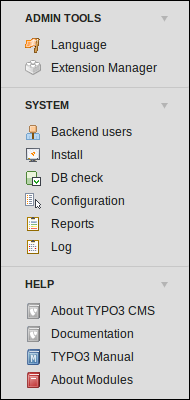
\includegraphics[width=0.35\linewidth]{Images/BackendChanges/AdminTools.png}
			\end{figure}
		\end{column}

	\end{columns}

\end{frame}

% ------------------------------------------------------------------------------
% Visual Appearance
% ------------------------------------------------------------------------------
% http://forge.typo3.org/issues/36017

\begin{frame}[fragile]
	\frametitle{Zmiany w panelu administracyjnym}
	\framesubtitle{Wygląd}

	\begin{itemize}
		\item \texttt{<h1>}-nagłówki w głównym obszarze korzystają konsekwentnie z czcionki TYPO3 "Share"
	\end{itemize}

	\begin{figure}
		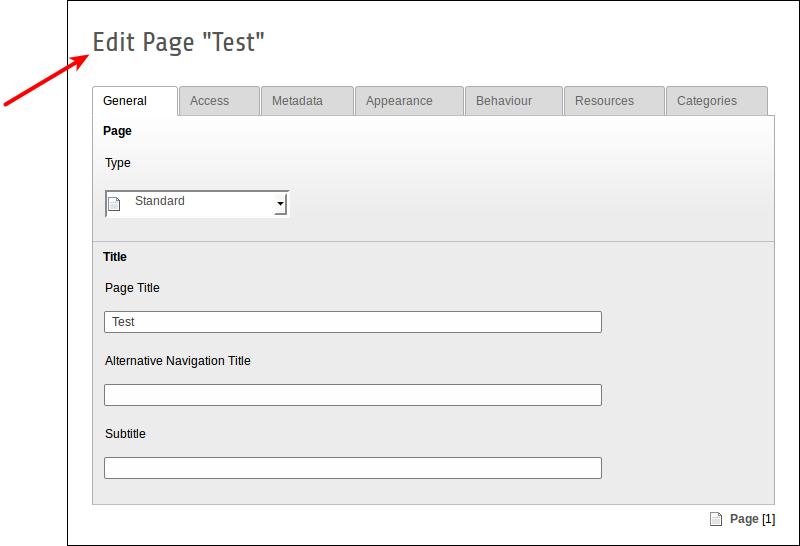
\includegraphics[width=0.6\linewidth]{Images/BackendChanges/ConsistantFont.png}
	\end{figure}

\end{frame}

% ------------------------------------------------------------------------------
% Visual Appearance
% ------------------------------------------------------------------------------
% http://forge.typo3.org/issues/41631

\begin{frame}[fragile]
	\frametitle{Zmiany w panelu administracyjnym}
	\framesubtitle{Wygląd}

	\begin{itemize}
		\item Moduł "Reports" ma nową ikonkę
	\end{itemize}

	\begin{figure}
		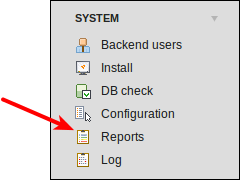
\includegraphics[width=0.35\linewidth]{Images/BackendChanges/ModuleReportsIcon.png}
	\end{figure}

\end{frame}

% ------------------------------------------------------------------------------
% Drag&Drop File Upload in Filelist (FAL)
% ------------------------------------------------------------------------------
% http://forge.typo3.org/issues/47005

\begin{frame}[fragile]
	\frametitle{Zmiany w panelu administracyjnym}
	\framesubtitle{Przesyłanie plików metodą Przeciągnij i Upuść (ang.Drag\&Drop) (1)}

	\begin{itemize}
		\item Udostępniona funkcjonalność przesyłania plików HTML5 Drag\&Drop w liście plików 

	\end{itemize}

	\begin{figure}
		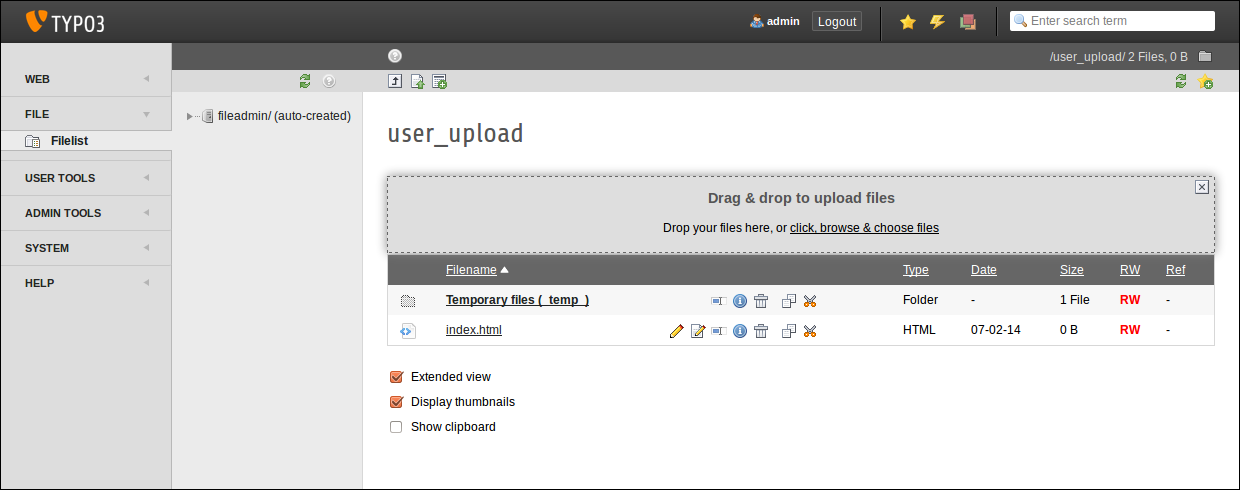
\includegraphics[width=0.95\linewidth]{Images/BackendChanges/DragDropFileUpload.png}
	\end{figure}

\end{frame}

% ------------------------------------------------------------------------------
% Drag&Drop File Upload Via Content Elements
% (slide added in March 2014)
% ------------------------------------------------------------------------------

\begin{frame}[fragile]
	\frametitle{Zmiany w panelu administracyjnym}
	\framesubtitle{Przesyłanie plików metodą Przeciągnij i Upuść (ang.Drag\&Drop) (2)}

	\begin{itemize}
		\item ...jak i przez elementy treści (przycisk: "Select \& upload files")

	\end{itemize}

	\begin{figure}
		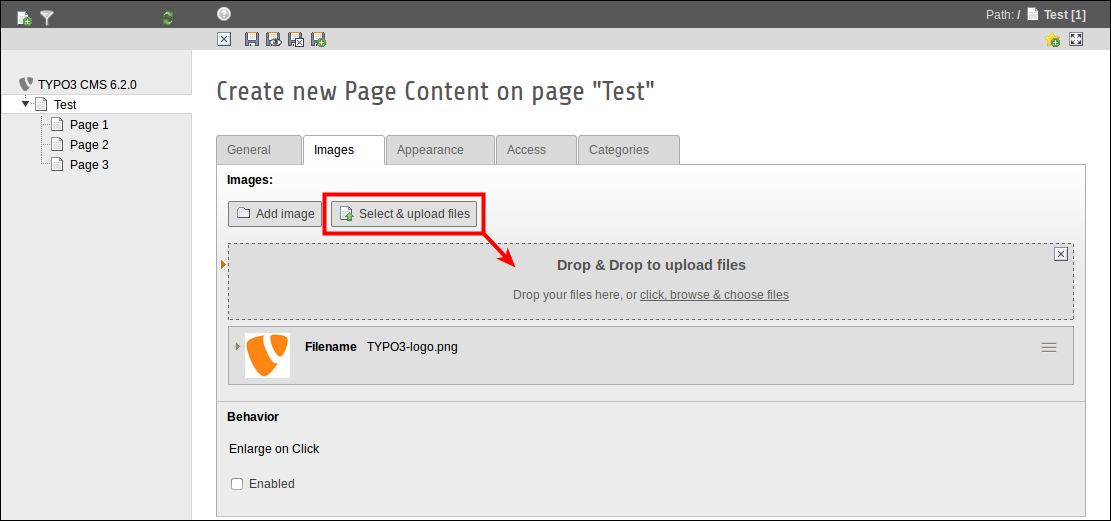
\includegraphics[width=0.95\linewidth]{Images/BackendChanges/SelectAndUploadFiles.png}
	\end{figure}

\end{frame}

% ------------------------------------------------------------------------------
% Backend Users
% ------------------------------------------------------------------------------
% http://forge.typo3.org/issues/43053

\begin{frame}[fragile]
	\frametitle{Zmiany w panelu administracyjnym}
	\framesubtitle{Użyteczność: Lista uzytkowników w panelu administracyjnym}

	\begin{itemize}
		\item Pokazana nazwa użytkownika, prawdziwe imię i nazwisko (pierwsza kolumna na liście)
		\item Kliknięcie na nazwę użytkownika (imię i nazwisko) edytuje dane użytkownika
		\item Dodany przycisk usuwania użytkownika z listy

	\end{itemize}

	\begin{figure}
		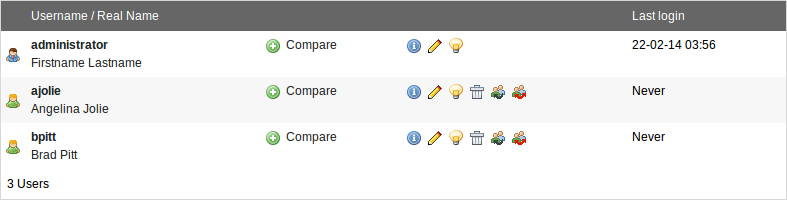
\includegraphics[width=0.95\linewidth]{Images/BackendChanges/BackendUserList.png}
	\end{figure}

\end{frame}

% ------------------------------------------------------------------------------
% Live Search
% ------------------------------------------------------------------------------
% http://forge.typo3.org/issues/35358

\begin{frame}[fragile]
	\frametitle{Zmiany w panelu administracyjnym}
	\framesubtitle{Wyszukiwanie z podpowiedziami (ang.autocompletion) }

	\begin{itemize}
		\item Tooltip pokazuje UID oraz PID w "livesearch"
		\item Po zakończeniu wyszukiwania formularz zostanie ponownie zamknięty i zostaje pokazany widok listy (na niepustej stronie)
	\end{itemize}

	\begin{figure}
		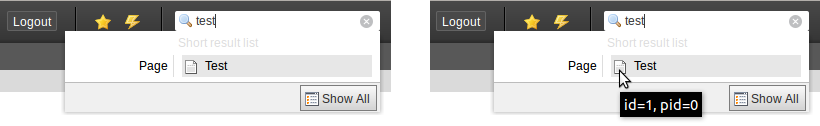
\includegraphics[width=0.8\linewidth]{Images/BackendChanges/LiveSearchTooltip.png}
	\end{figure}

\end{frame}

% ------------------------------------------------------------------------------
% Live Search
% ------------------------------------------------------------------------------

\begin{frame}[fragile]
	\frametitle{Zmiany w panelu administracyjnym}
	\framesubtitle{Wyszukiwanie z podpowiedziami (ang.autocompletion) }

	\begin{itemize}
		\item W TYPO3 < 6.2, dla stron, pod uwagę są brane tylko kolumny tabel \texttt{title} i \texttt{uid}
		\item W TYPO3 >= 6.2, pola \texttt{alias} mogą być dodawane do wyszukiwania\newline
			(wymaga UserTSconfig: \texttt{options.pageTree.searchInAlias = 1})
	\end{itemize}

	\begin{figure}
		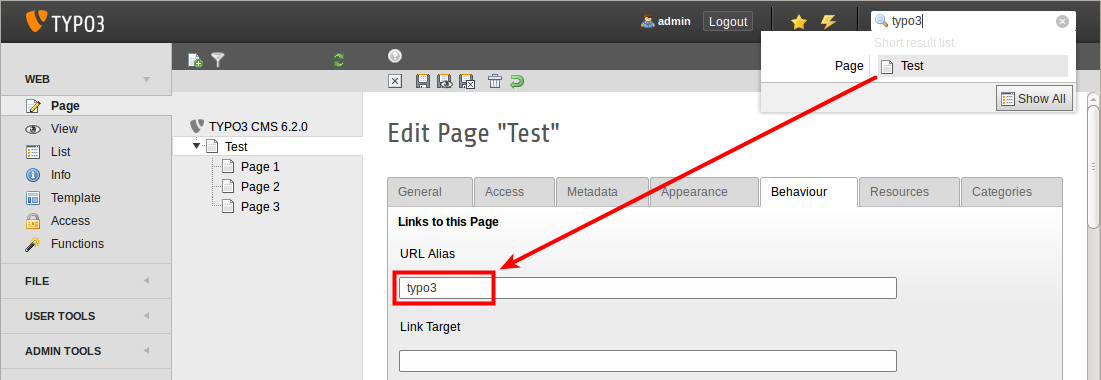
\includegraphics[width=0.95\linewidth]{Images/BackendChanges/LiveSearchInAlias.png}
	\end{figure}

\end{frame}

% ------------------------------------------------------------------------------
% File Abstraction Layer
% ------------------------------------------------------------------------------

\begin{frame}[fragile]
	\frametitle{Zmiany w panelu administracyjnym}
	\framesubtitle{Warstwa Abstrakcyjna Pliku}

	\begin{itemize}
		\item Tytuł i nazwa pliku w nagłówku WAP
	\end{itemize}

	\begin{figure}
		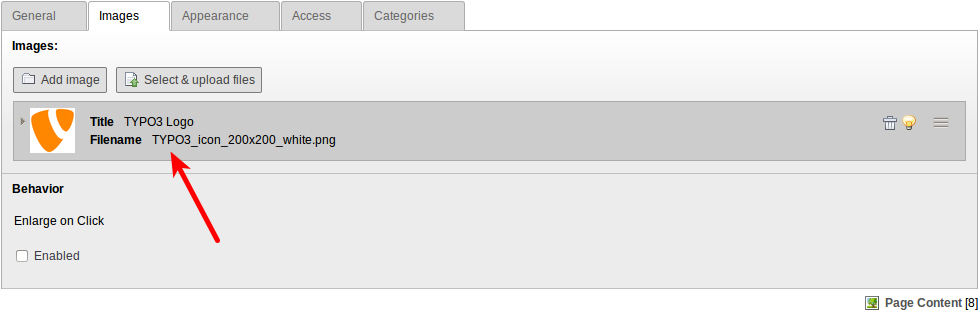
\includegraphics[width=0.95\linewidth]{Images/BackendChanges/FalTitleAndFilename.png}
	\end{figure}

\end{frame}

% ------------------------------------------------------------------------------
% File Abstraction Layer
% ------------------------------------------------------------------------------

\begin{frame}[fragile]
	\frametitle{Zmiany w panelu administracyjnym}
	\framesubtitle{Warstwa Abstrakcyjna Pliku (EXT:filemetadata)}

	\begin{itemize}
		\item Rozszerzenie systemowe "filemetadata" dodaje nowe zakładki aby wyświetlić dane meta\newline
			\small(rozszerzenie jest ładowane wraz z jądrem, ale nie jest domyślnie zainstalowane)\normalsize
	\end{itemize}

	\begin{figure}
		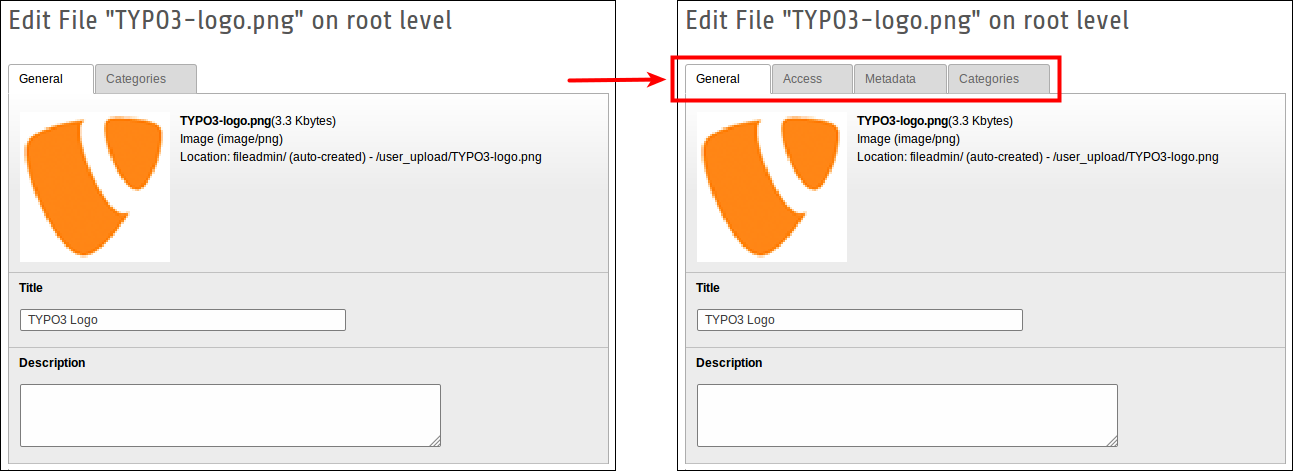
\includegraphics[width=0.8\linewidth]{Images/BackendChanges/FileMetaDataTabs.png}
	\end{figure}

\end{frame}

% ------------------------------------------------------------------------------
% File Abstraction Layer
% ------------------------------------------------------------------------------

\begin{frame}[fragile]
	\frametitle{Zmiany w panelu administracyjnym}
	\framesubtitle{Warstwa Abstrakcyjna Pliku (EXT:filemetadata)}

	\begin{figure}
		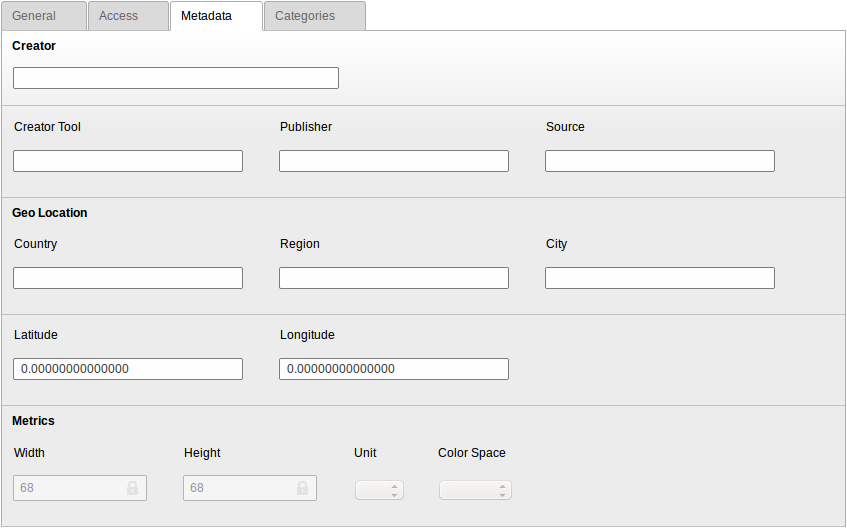
\includegraphics[width=0.8\linewidth]{Images/BackendChanges/FileMetaData.png}
	\end{figure}

\end{frame}

% ------------------------------------------------------------------------------
% File Abstraction Layer
% ------------------------------------------------------------------------------

\begin{frame}[fragile]
	\frametitle{Zmiany w panelu administracyjnym}
	\framesubtitle{Warstwa Abstrakcyjna Pliku}

	\begin{itemize}
		\item Możliwość tłumaczenia danych meta WAP na język lokalizacji strony.
	\end{itemize}

	\begin{figure}
		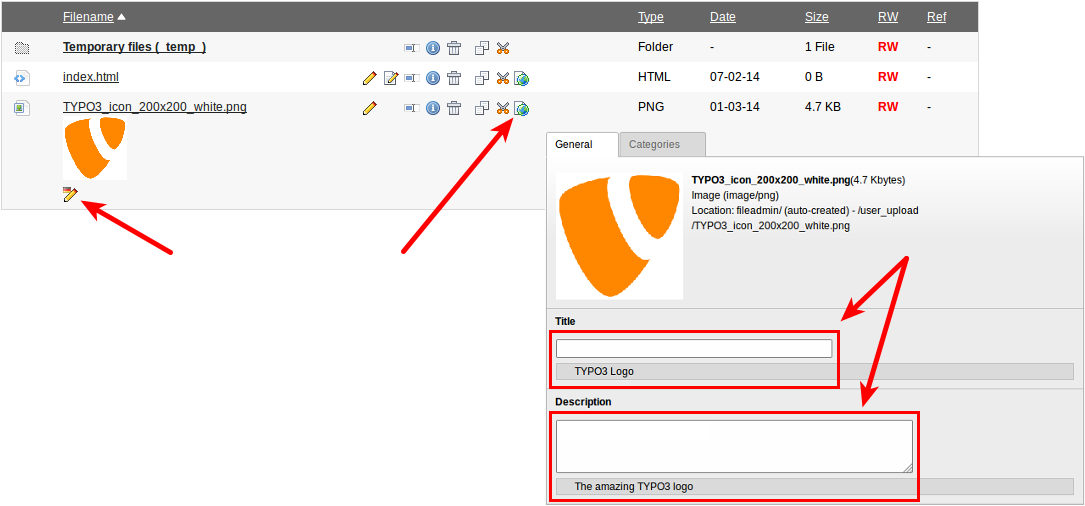
\includegraphics[width=0.95\linewidth]{Images/BackendChanges/FalTranslateMetaData.png}
	\end{figure}

\end{frame}

% ------------------------------------------------------------------------------
% Module: Documentation
% ------------------------------------------------------------------------------

\begin{frame}[fragile]
	\frametitle{Zmiany w panelu administracyjnym}
	\framesubtitle{Moduł: Documentation}

	\begin{columns}[T]

		\begin{column}{.5\textwidth}
			\begin{itemize}
				\item Moduł "Documentation" pozwala użytkownikom panelu administracyjnego pobierać lub oglądać instrukcje
				\item Nowe instalacje TYPO3 wczytują ten moduł domyślnie
				\item Funkcja "Download Documentation" pobiera instrukcje (spójrz na ilustrację)
				\item Użyj Menadżera Rozszerzeń aby wczytać "Documentation" na zaktualizowanej instalacji TYPO3
			\end{itemize}
		\end{column}

		\begin{column}{.5\textwidth}
			\begin{figure}\vspace*{-0.4cm}
				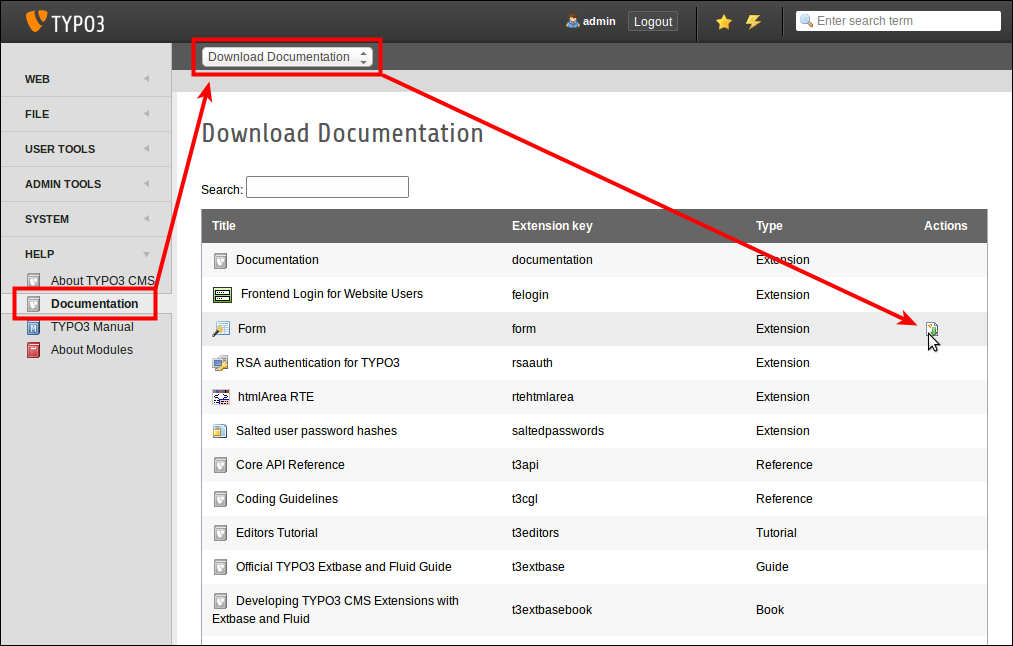
\includegraphics[width=1\linewidth]{Images/BackendChanges/DownloadDocumentation.png}
			\end{figure}
		\end{column}

	\end{columns}

\end{frame}

% ------------------------------------------------------------------------------
% Module: Documentation
% ------------------------------------------------------------------------------

\begin{frame}[fragile]
	\frametitle{Zmiany w panelu administracyjnym}
	\framesubtitle{Moduł: Documentation}

	\begin{itemize}
		\item Funkcja "Show Documentation" wyświetla pobrane instrukcje
	\end{itemize}

	\begin{figure}
		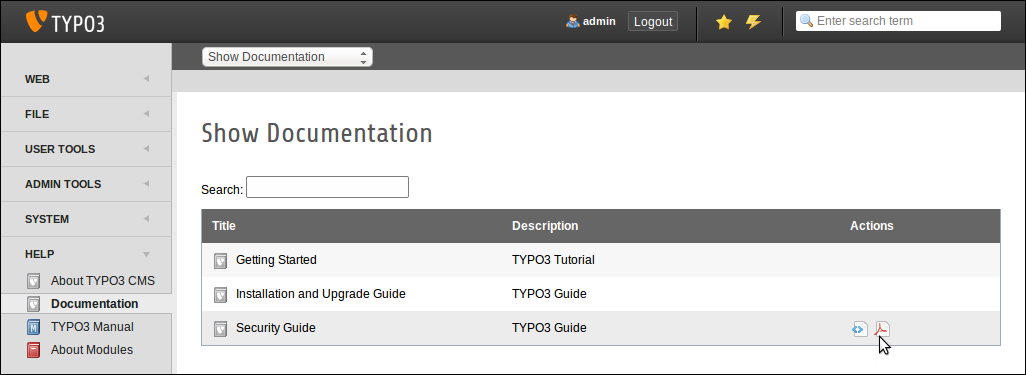
\includegraphics[width=0.95\linewidth]{Images/BackendChanges/ShowDocumentation.png}
	\end{figure}

\end{frame}

% ------------------------------------------------------------------------------
% Removed: TypoScript Help
% ------------------------------------------------------------------------------
% http://forge.typo3.org/issues/47931

\begin{frame}[fragile]
	\frametitle{Zmiany w panelu administracyjnym}
	\framesubtitle{Usunięte: TypoScript Help}

 	\begin{itemize}
		\item EXT:tsconfig\_help ("TSconfig Quick Reference") usunięte\newline
			\small(nieaktualne informacje nie aktualizowane od TYPO3 CMS 4.1)
	\end{itemize}

	\begin{figure}
		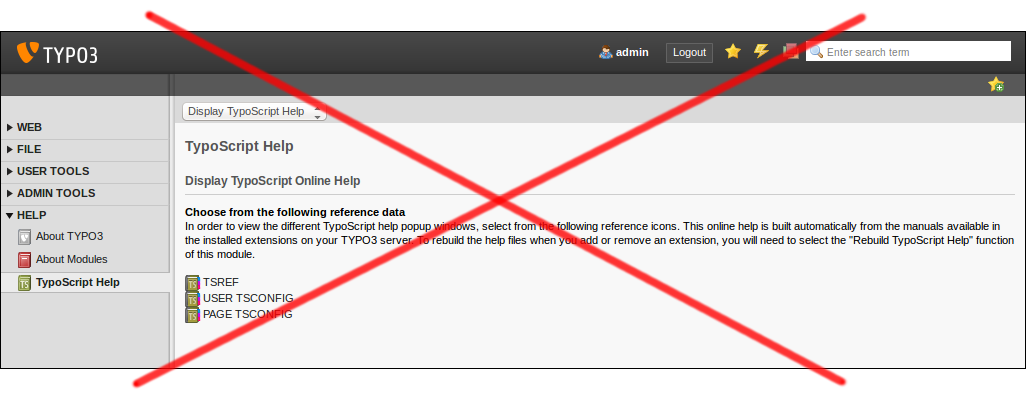
\includegraphics[width=0.95\linewidth]{Images/BackendChanges/TypoScriptHelpRemovedCrossed.png}
	\end{figure}

\end{frame}


% ------------------------------------------------------------------------------
% Scheduler
% ------------------------------------------------------------------------------

\begin{frame}[fragile]
	\frametitle{Zmiany w panelu administracyjnym}
	\framesubtitle{Planowanie zadań}
	\begin{itemize}
		\item Możliwość usunięcia zadania z poziomu widoku edycji \newline
			\small(w TYPO3 < 6.2, funkcja usuwania była dostępna tylko w widoku listy)\normalsize
	\end{itemize}

	\begin{figure}
		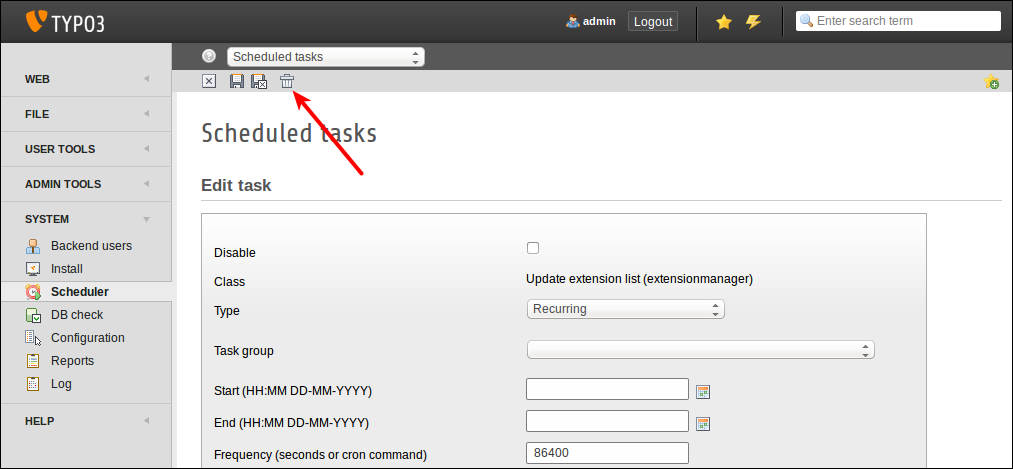
\includegraphics[width=0.95\linewidth]{Images/BackendChanges/DeleteSchedulerTaskInEditView.png}
	\end{figure}

\end{frame}

% ------------------------------------------------------------------------------
% Scheduler
% ------------------------------------------------------------------------------

\begin{frame}[fragile]
	\frametitle{Zmiany w panelu administracyjnym}
	\framesubtitle{Planowanie zadań}

	\begin{itemize}
		\item Opis może być przypisany do zadań harmonogramu i pokazany jako krótki nagłówek w widoku listy lub jako tooltip (zobacz następny slajd)
	\end{itemize}

	\begin{figure}
		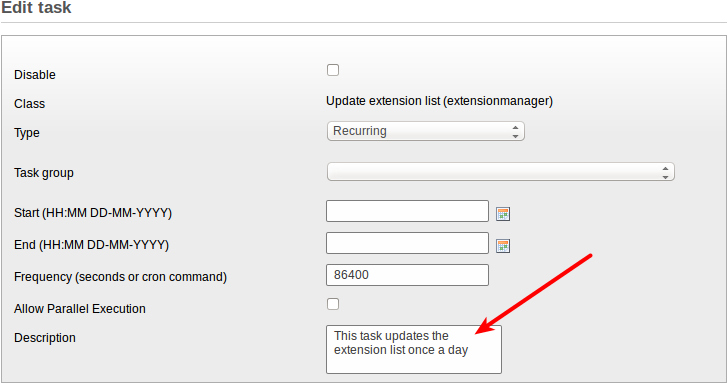
\includegraphics[width=0.7\linewidth]{Images/BackendChanges/SchedulerTaskDescription.png}
	\end{figure}

\end{frame}

% ------------------------------------------------------------------------------
% Scheduler
% ------------------------------------------------------------------------------

\begin{frame}[fragile]
	\frametitle{Zmiany w panelu administracyjnym}
	\framesubtitle{Planowanie zadań}

	\begin{itemize}
		\item Opis zadania jako krótki nagłówek\newline
			\small(ta właściwość musi być aktywowana w konfiguracji rozszerzeń)\normalsize
	\end{itemize}

	\begin{figure}
		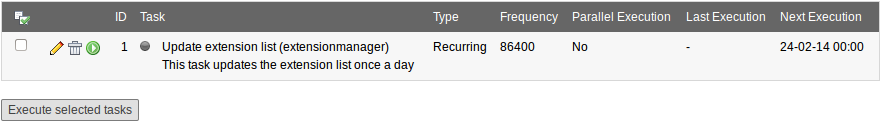
\includegraphics[width=0.95\linewidth]{Images/BackendChanges/SchedulerTaskDescriptionAsSubheader.png}
	\end{figure}

	\begin{itemize}
		\item Opis zadania jako tooltip ("hover")
	\end{itemize}

	\begin{figure}
		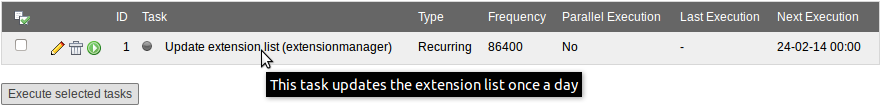
\includegraphics[width=0.95\linewidth]{Images/BackendChanges/SchedulerTaskDescriptionAsTooltip.png}
	\end{figure}

\end{frame}

% ------------------------------------------------------------------------------
% Scheduler
% ------------------------------------------------------------------------------

\begin{frame}[fragile]
	\frametitle{Zmiany w panelu administracyjnym}
	\framesubtitle{Planowanie zadań}

	\begin{itemize}
		\item Możliwość grupowania zadań
		\item Dodaj rekordy "scheduler task group" do strony źródłowej (UID: 0)\newline
			i wybierz grupę w edycji zadania
	\end{itemize}

	\begin{figure}
		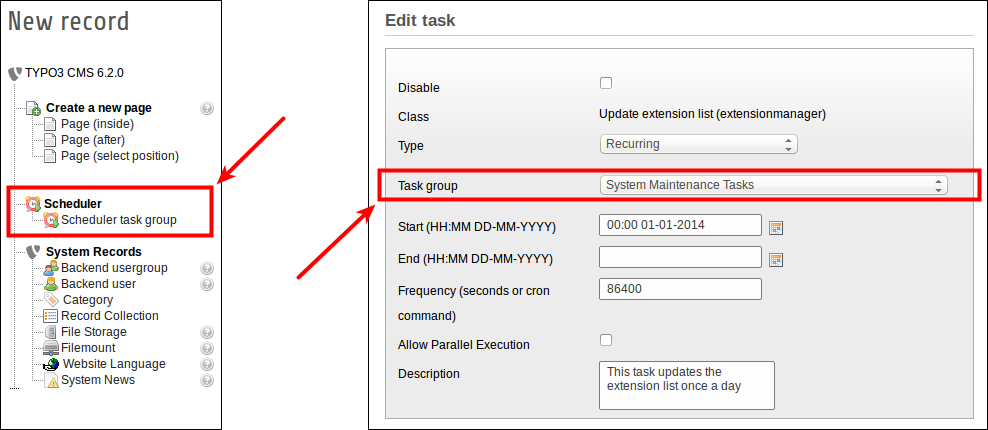
\includegraphics[width=0.85\linewidth]{Images/BackendChanges/SchedulerTaskGroup.png}
	\end{figure}

\end{frame}

% ------------------------------------------------------------------------------
% System Extension: Form
% ------------------------------------------------------------------------------
% http://forge.typo3.org/issues/38094

\begin{frame}[fragile]
	\frametitle{Zmiany w panelu administracyjnym}
	\framesubtitle{Rozszerzenia Systemowe: Form}

	\begin{columns}[T]

		\begin{column}{.5\textwidth}
			\begin{itemize}
				\item Nowy postprocesor dla cObject FORM: \textbf{redirect}\newline
					(przekierowuje po zapisaniu formularza)
				\item Wartość jest parsowana przez \texttt{typolink} (funkcja TypoScript),\newline
					co oznacza, że może być zarówno ID strony jak i URL-em
			\end{itemize}
		\end{column}

		\begin{column}{.5\textwidth}
			\begin{figure}\vspace*{-0.4cm}
				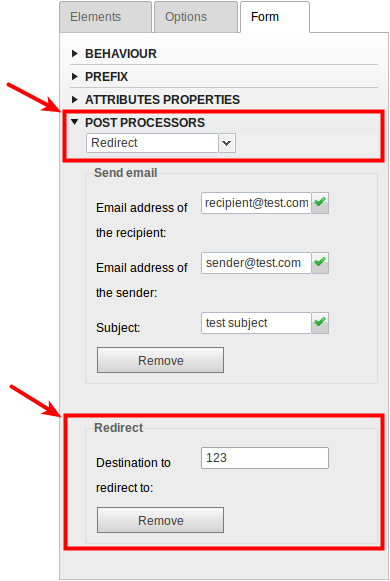
\includegraphics[width=0.65\linewidth]{Images/BackendChanges/FormRedirectPostProcessor.png}
			\end{figure}
		\end{column}

	\end{columns}

\end{frame}

% ------------------------------------------------------------------------------
% Module: List
% ------------------------------------------------------------------------------
% http://forge.typo3.org/issues/49810

\begin{frame}[fragile]
	\frametitle{Zmiany w panelu administracyjnym}
	\framesubtitle{Lista modułów}

	\begin{itemize}
		\item Dodatkowe kolumny "UID" i "PID" w widoku listy dla wszystkich użytkowników
	\end{itemize}

	\begin{figure}
		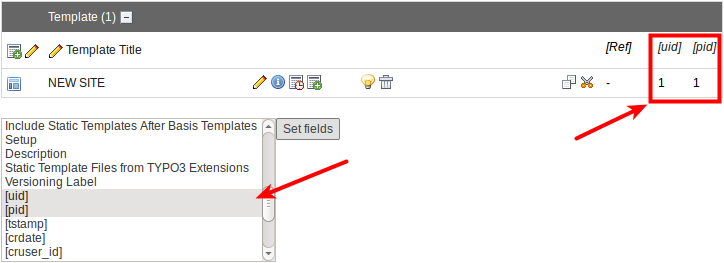
\includegraphics[width=0.95\linewidth]{Images/BackendChanges/AdditionalColumnsInListModule.png}
	\end{figure}

\end{frame}

% ------------------------------------------------------------------------------
% File Abstraction Layer
% ------------------------------------------------------------------------------
% http://forge.typo3.org/issues/50827
% http://forge.typo3.org/issues/51097

\begin{frame}[fragile]
	\frametitle{Zmiany w panelu administracyjnym}
	\framesubtitle{Warstwa Abstrakcyjna Pliku}

	\begin{itemize}
		\item Jeżeli plik nie zostanie odnaleziony, pojawi się informacja i zostanie ustawiona flaga dla rekordu w bazie danych
		\item Moduł "Reports" wykazuje to jako problem
		\item Jeżeli plik pojawi się ponownie, wiadomość i flaga zostaną zresetowane
	\end{itemize}

	\begin{columns}[T]

		\begin{column}{.5\textwidth}
			\begin{figure}
				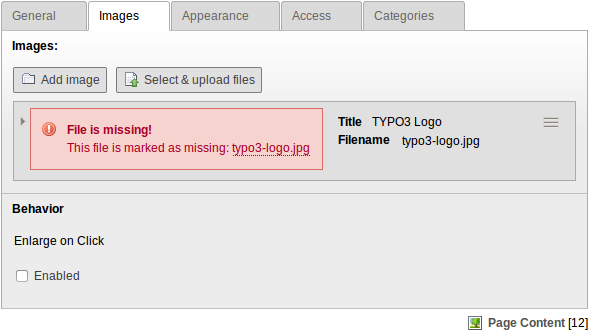
\includegraphics[width=0.95\linewidth]{Images/BackendChanges/FalMissingFileContentElement.png}
			\end{figure}
		\end{column}

		\begin{column}{.5\textwidth}
			\begin{figure}
				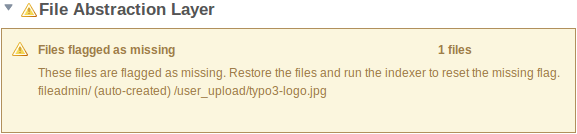
\includegraphics[width=0.95\linewidth]{Images/BackendChanges/FalMissingFileReportsModule.png}
			\end{figure}
		\end{column}

	\end{columns}

\end{frame}

% ------------------------------------------------------------------------------
% Menu/Sitemap: Category-based Menus
% ------------------------------------------------------------------------------
% http://forge.typo3.org/issues/51161

\begin{frame}[fragile]
	\frametitle{Zmiany w panelu administracyjnym}
	\framesubtitle{Menu oparte na kategoriach (1)}

	\begin{itemize}
		\item Element treści "Menu/Sitemap" może stworzyć menu oparte na kategoriach
	\end{itemize}

	\begin{figure}
		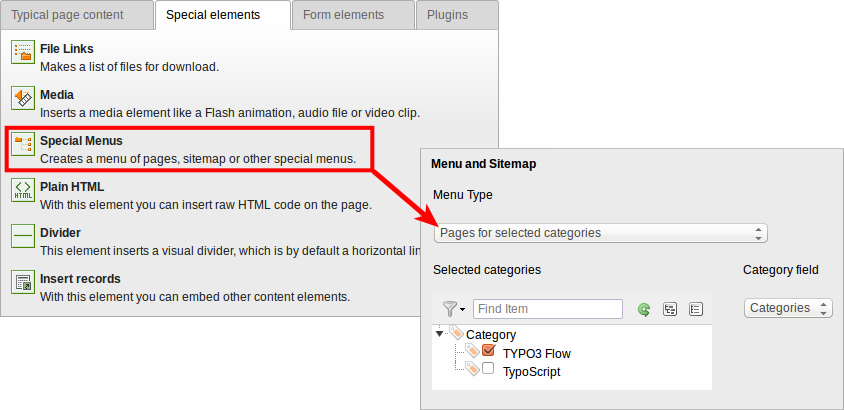
\includegraphics[width=0.8\linewidth]{Images/BackendChanges/CategoryBasedMenus.png}
	\end{figure}

\end{frame}

% ------------------------------------------------------------------------------
% Menu/Sitemap: Category-based Menus
% (slide added in March 2014)
% ------------------------------------------------------------------------------

\begin{frame}[fragile]
	\frametitle{Zmiany w panelu administracyjnym}
	\framesubtitle{Menu oparte na kategoriach (2)}

	\begin{itemize}
		\item Kolejny nowy typ menu: "\underline{Content elements} for selected categories"
	\end{itemize}

	\begin{figure}
		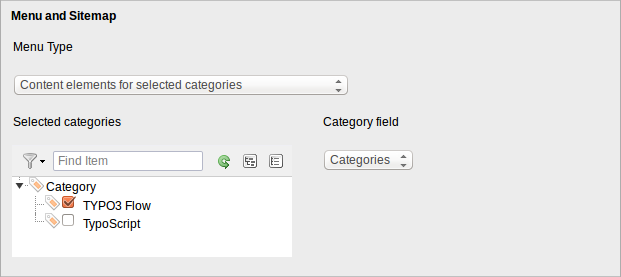
\includegraphics[width=0.6\linewidth]{Images/BackendChanges/ContentElementsForSelectedCategories.png}
	\end{figure}

\end{frame}

% ------------------------------------------------------------------------------
% Sorting Categories
% ------------------------------------------------------------------------------
% http://forge.typo3.org/issues/51590

\begin{frame}[fragile]
	\frametitle{Zmiany w panelu administracyjnym}
	\framesubtitle{Sortowanie kategorii}

 	\begin{itemize}
		\item Teraz kategorie mogą być sortowane\newline
			\small(w TYPO3 < 6.2, kategorie zawsze są sortowane alfabetycznie)\normalsize
	\end{itemize}

	\begin{figure}
		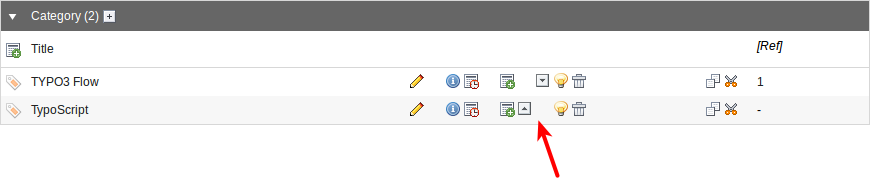
\includegraphics[width=0.95\linewidth]{Images/BackendChanges/CategorySorting.png}
	\end{figure}

\end{frame}

% ------------------------------------------------------------------------------
% Category Visibility
% ------------------------------------------------------------------------------
% http://forge.typo3.org/issues/52718

\begin{frame}[fragile]
	\frametitle{Zmiany w panelu administracyjnym}
	\framesubtitle{Widoczność kategorii}

 	\begin{itemize}
		\item Widoczność kategorii może być ograniczona dla użytkowników/grup w panelu administracyjnym
	\end{itemize}

	\begin{figure}
		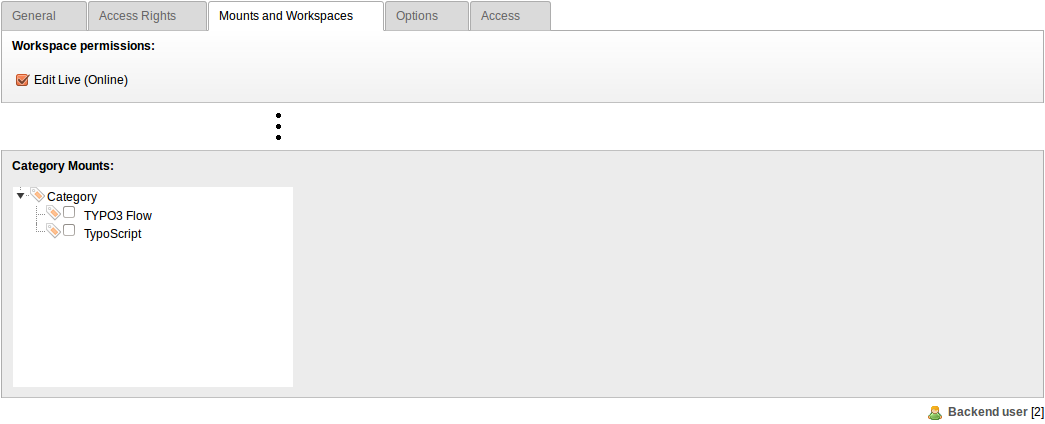
\includegraphics[width=0.95\linewidth]{Images/BackendChanges/CategoryVisibility.png}
	\end{figure}

\end{frame}

% ------------------------------------------------------------------------------
% "New Content" icon always visible
% ------------------------------------------------------------------------------
% http://forge.typo3.org/issues/48938
% http://forge.typo3.org/issues/51480

\begin{frame}[fragile]
	\frametitle{Zmiany w panelu administracyjnym}
	\framesubtitle{Uzyteczność}

 	\begin{itemize}
		\item Ikona "new content" jest zawsze widoczna jeśli kolumna jest pusta\newline
			\small(pomaga to zrozumieć edytującym co mogą robić)\normalsize
	\end{itemize}

	\begin{figure}
		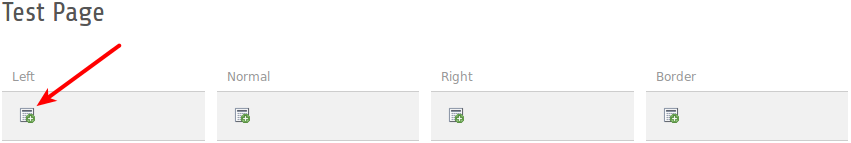
\includegraphics[width=0.95\linewidth]{Images/BackendChanges/NewContentIconAlwaysVisible.png}
	\end{figure}

\end{frame}

% ------------------------------------------------------------------------------
% Module "Functions": Hide In Menus
% ------------------------------------------------------------------------------
% http://forge.typo3.org/issues/51017

\begin{frame}[fragile]
	\frametitle{Zmiany w panelu administracyjnym}
	\framesubtitle{Funkcje}

 	\begin{itemize}
		\item Kiedy edytujący tworzą wielokrotne strony w module "functions", nowe pole wyboru pozwala im ukryć te strony w menu\newline
			\small(bardzo przydatne podczas tworzenia wielu stron jednocześnie)\normalsize
	\end{itemize}

	\begin{figure}
		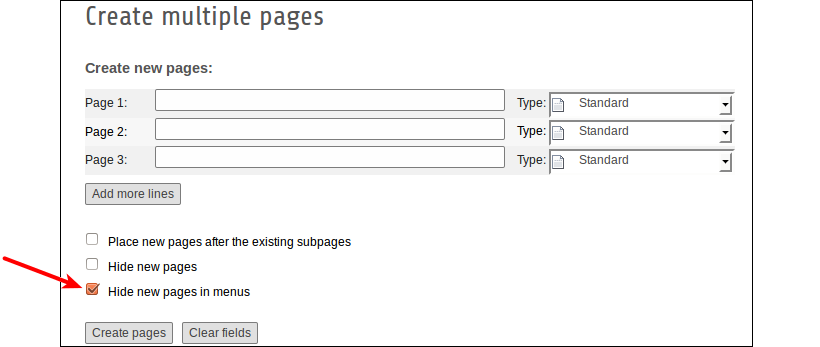
\includegraphics[width=0.85\linewidth]{Images/BackendChanges/CreateMultiplePagesHideInMenu.png}
	\end{figure}

\end{frame}

% ------------------------------------------------------------------------------
% Extension Manager: Upload Extensions
% ------------------------------------------------------------------------------
% http://forge.typo3.org/issues/51776
% http://forge.typo3.org/issues/51437

\begin{frame}[fragile]
	\frametitle{Zmiany w panelu administracyjnym}
	\framesubtitle{Menadzer Rozszerzeń}

 	\begin{itemize}
		\item Przesyłanie modułów poprzez funkcję "Get Extensions"
	\end{itemize}

	\begin{figure}
		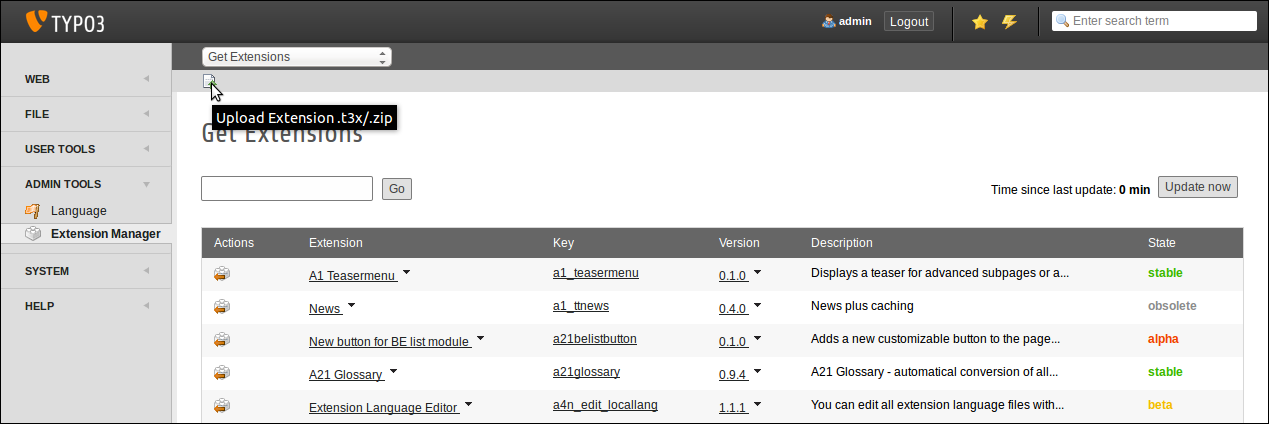
\includegraphics[width=0.95\linewidth]{Images/BackendChanges/UploadExtension.png}
	\end{figure}

\end{frame}

% ------------------------------------------------------------------------------
% Recycler
% ------------------------------------------------------------------------------
% http://forge.typo3.org/issues/52324

\begin{frame}[fragile]
	\frametitle{Zmiany w panelu administracyjnym}
	\framesubtitle{Recykler}

 	\begin{itemize}
		\item Rekordy recyklera mogą być sortowane według znacznika czasu\newline
			\small(pomaga to użytkownikom zdecydować czy odzyskać właściwy rekord czy nie)\normalsize
	\end{itemize}

	\begin{figure}
		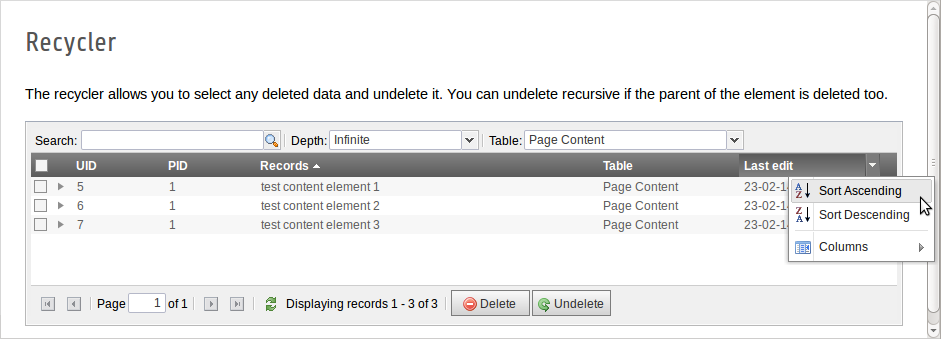
\includegraphics[width=0.95\linewidth]{Images/BackendChanges/RecyclerSortRecord.png}
	\end{figure}

\end{frame}

% ------------------------------------------------------------------------------
% File/Directory Permissions
% ------------------------------------------------------------------------------

\begin{frame}[fragile]
	\frametitle{Zmiany w panelu administracyjnym}
	\framesubtitle{Uprawnienia plików/katalogów}

 	\begin{itemize}
		\item Bardziej szczegółowe uprawnienia plików/katalogów dla użytkowników/grup w panelu administracyjnym 
			\begingroup\color{typo3red}\textbf{(1)}\endgroup
		\item Jest to możliwe od TYPO3 6.0, lecz tylko przez UserTSconfig
			\begingroup\color{typo3red}\textbf{(2)}\endgroup
	\end{itemize}

	\begin{figure}
		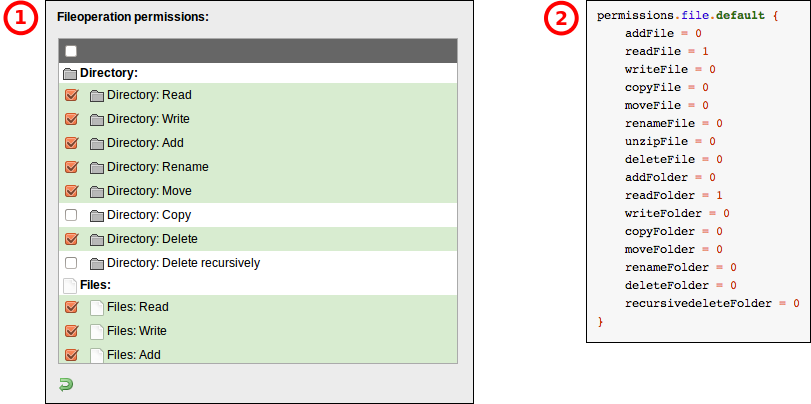
\includegraphics[width=0.75\linewidth]{Images/BackendChanges/FileAndDirectoryPermissions.png}
	\end{figure}

\end{frame}

% ------------------------------------------------------------------------------
% OpenID
% ------------------------------------------------------------------------------

\begin{frame}[fragile]
	\frametitle{Zmiany w panelu administracyjnym}
	\framesubtitle{OpenID (1)}

 	\begin{itemize}
		\item OpenID do autoryzacji użytkowników panelu administracyjnego można skonfigurować za pomocą kreatora
		\item EXT:openid (rozszerzenie systemowe) jest wymagane przez tę funkcję
	\end{itemize}

	\begin{figure}
		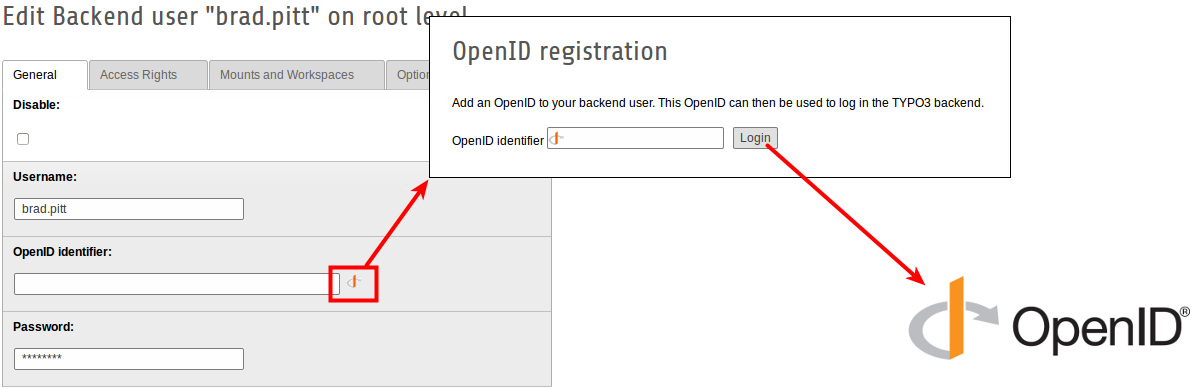
\includegraphics[width=0.95\linewidth]{Images/BackendChanges/OpenIdWizard.png}
	\end{figure}

\end{frame}

% ------------------------------------------------------------------------------
% OpenID
% ------------------------------------------------------------------------------

\begin{frame}[fragile]
	\frametitle{Zmiany w panelu administracyjnym}
	\framesubtitle{OpenID (2)}

 	\begin{itemize}
		\item OpenID do autoryzacji użytkowników panelu administracyjnego można skonfigurować za pomocą kreatora
		\item EXT:openid (rozszerzenie systemowe) jest wymagane przez tę funkcję
	\end{itemize}

	\begin{figure}
		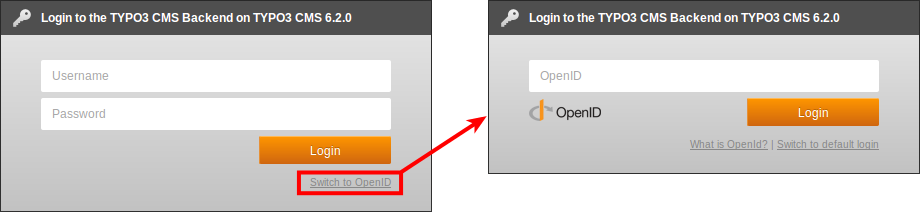
\includegraphics[width=0.8\linewidth]{Images/BackendChanges/OpenIdLogin.png}
	\end{figure}

 	\begin{itemize}
		\item Więcej informacji o OpenID:\newline
			\small\url{http://openid.net}\normalsize
	\end{itemize}

\end{frame}

% ------------------------------------------------------------------------------
% Workspaces
% ------------------------------------------------------------------------------
% http://forge.typo3.org/issues/50223
% http://forge.typo3.org/issues/50224

\begin{frame}[fragile]
	\frametitle{Zmiany w panelu administracyjnym}
	\framesubtitle{Obszary robocze}

 	\begin{itemize}
		\item Edytorzy/użytkownicy mogą zdefiniować kogo zawiadomić, bez ograniczania tego na poziomie systemu
		\item Zakładka "All" jest teraz widoczna dla \underline{wszystkich} użytkowników
	\end{itemize}

	\begin{figure}
		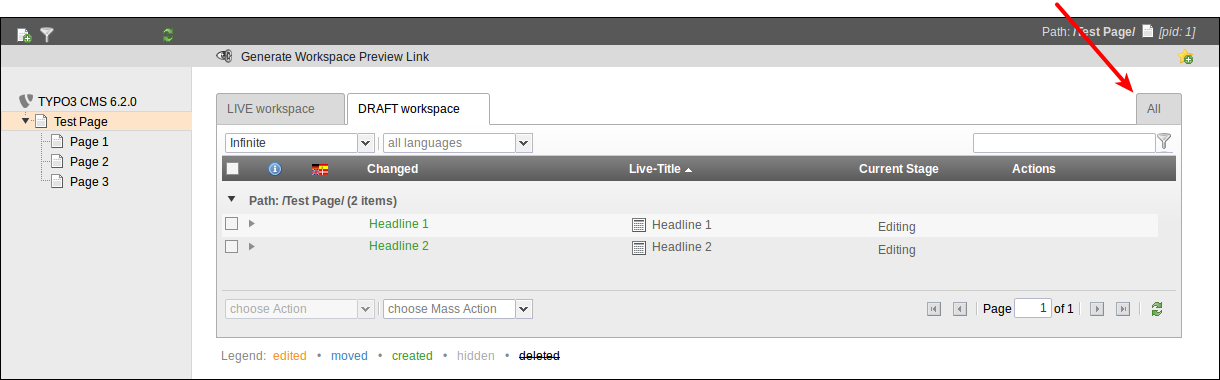
\includegraphics[width=0.95\linewidth]{Images/BackendChanges/WorkspacesTabAll.png}
	\end{figure}

\end{frame}

% ------------------------------------------------------------------------------

